\section{Project Design and Development Logic}
\label{frPMgantt}
Since \ac{FLAMeS} mission is an earth observation mission the main stakeholders researchers and the scientific community. They are the main drivers for the requirements of the mission. It is the challenge for the project engineers to translate those requirements into a working satellite system. One of the key features of the mission is to use a formation of mostly identical satellites, which eases the mission development and design compared to a mission with nine unique satellites. 

Both different types of satellites can be developed in parallel, since apart from the receiver instrument and the communication link the satellite designs are completely independent of each other. The fact that the design of the receiver satellites is based on the cubesat standard will reduce the time of the development considerably as well, since a lot of technology and components are standardised and available off the shelf. The testing equipment and infrastructure can be reused and will not have to be custom-made for every single satellite in the formation. 

Most of the basic satellite components used for the design of the emitter satellite are \ac{COTS} as well, which shortens the development and qualification time for that satellite. Most of the development time and cost will have to be put into the detailed design of the payloads, which are specialised instruments dedicated to this mission. Another critical part of the mission is the redesign of the rocket's upper stage to make it able to put all satellites in their own orbit.

A fast development time saves resources and will enable the mission to be launched in the spring of 2017. This way the measurements can be made at solar minimum and the least amount of propellant is needed for station keeping and orbital manoeuvres.

\section{Project Gantt Chart}
Naturally the \ac{FLAMeS} mission will extent a lot further in time than just the this feasibility study. To keep the mission on track until and beyond the launch a Gantt chart is set up for the project.

After the feasibility study is finished the precise mission definition is performed. When the exact requirements for all subsystems are known the detailed design can start. As soon as the design is fixed for different subsystems production and assembly of the subsystems can start. Even during while the production is still in progress the acceptance testing of the finished components and representative mock-ups can take place. This way design mistakes or production errors can be discovered early and problematic parts can be fixed or even redesigned. When all parts are finalised and tested the satellite can be integrated and transported to the launch site. When the satellite is put on the launcher the launch can commence.

After launch first the satellites need to be put in their correct orbits and the instruments are calibrated. Then the real mission can start and measurements are made. As soon as data is collected and send to the ground, researchers can start analysing the data and producing and publishing results. 

The Gantt chart can be found in figure \ref{ganttchart} on page \pageref{ganttchart}.

\begin{figure}
\centering
%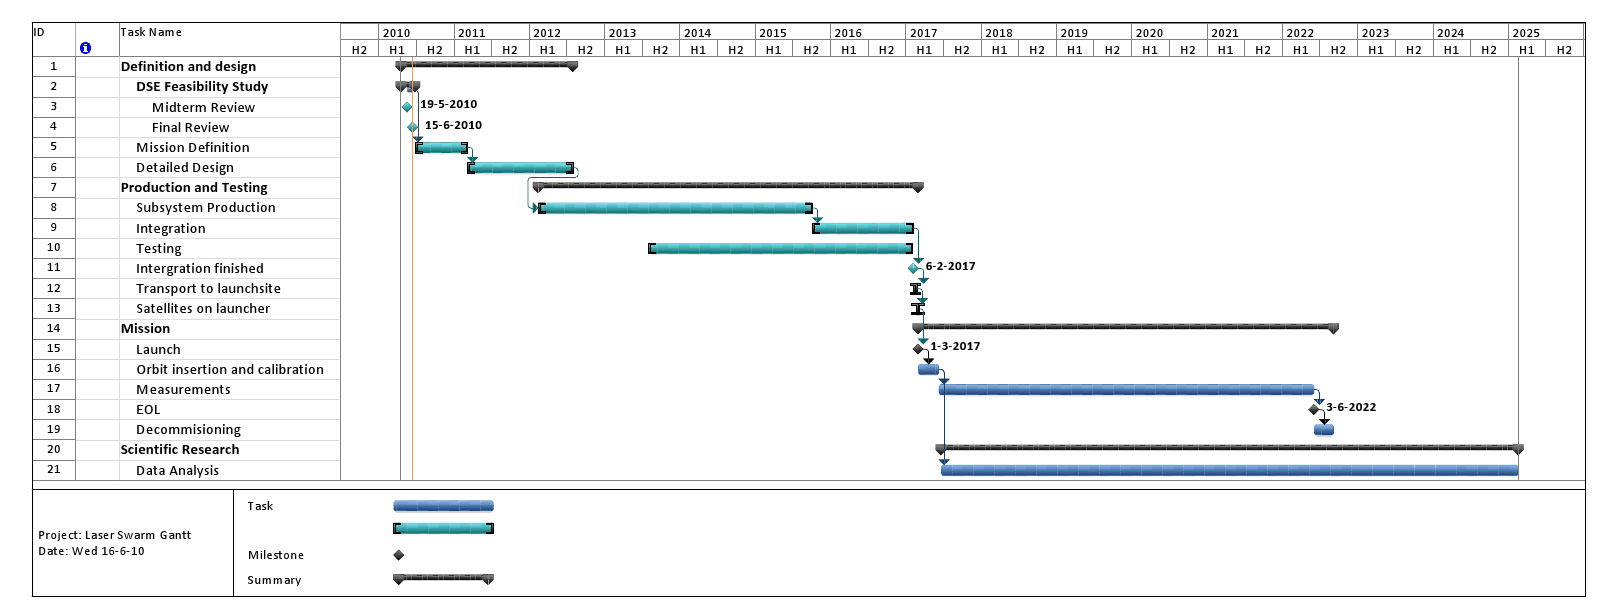
\includegraphics[width=0.8\textwidth, angle=90]{chapters/img/projectganttchart.png}
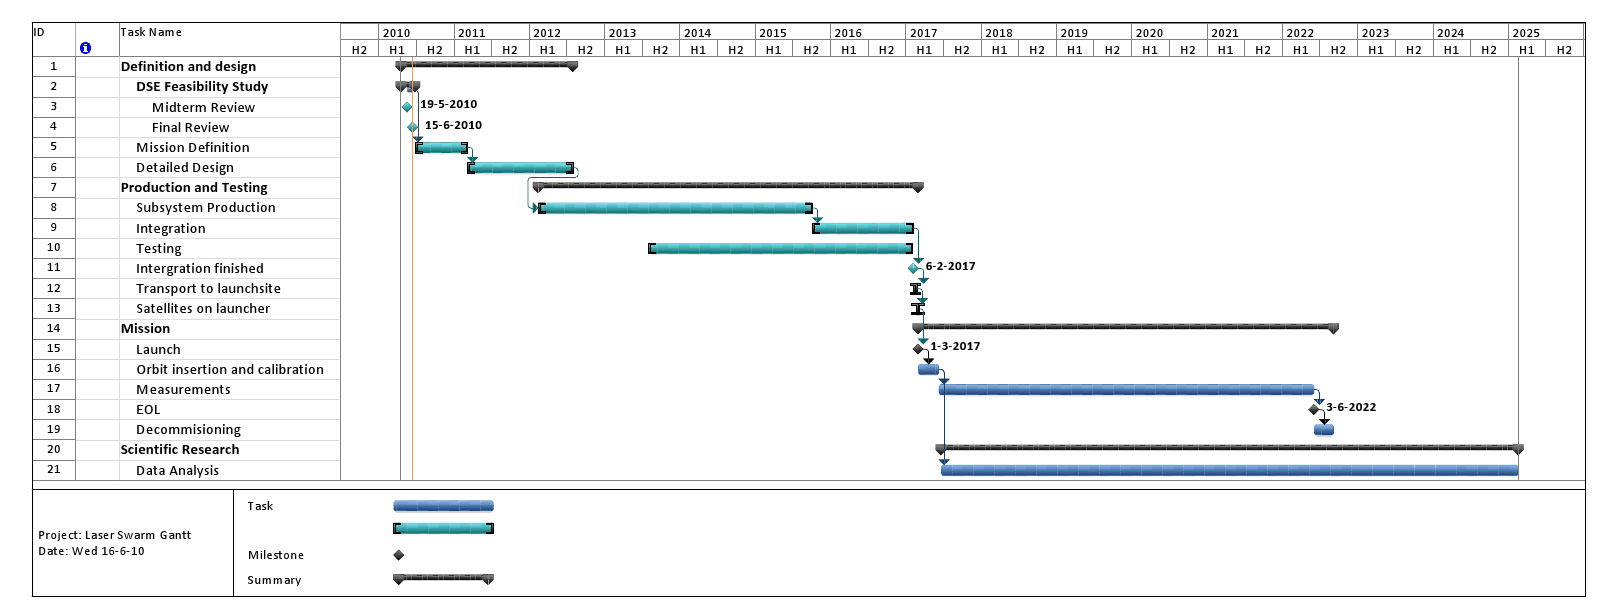
\includegraphics[width=1.3\textwidth, angle=90]{chapters/img/projectganttchart.png}
\caption{Project Gantt Chart}
\label{ganttchart}
\end{figure}